\section{Theorie}
\label{sec:Theorie}

\subsection{Motivation}

Wird eine Metalloberfläche mit Licht bestrahlt, ist es möglich Elektronen aus dem Metall zu lösen.
Dieser Effekt, welcher neben Compton-Effekt und Paarbildung eine quantenmechanische Sichtweise auf Licht fordert, wird als Photoeffekt bezeichnet.
Eine qualitative Erklärung des Photoeffektes lieferte Einstein im Jahre 1905, wofür er jedoch erst 1921 den Nobelpreis für Physik erhielt. \cite{skript}

\subsection{Erklärung des Photoeffektes}
Zur Untersuchung des Photoeffektes wird in einem einfachen Fall eine Photozelle benutzt, wie sie in Abbildung \ref{abb:1} in einem einfachen Stromkreis dargestellt ist.

\begin{figure}[H]
  \centering
  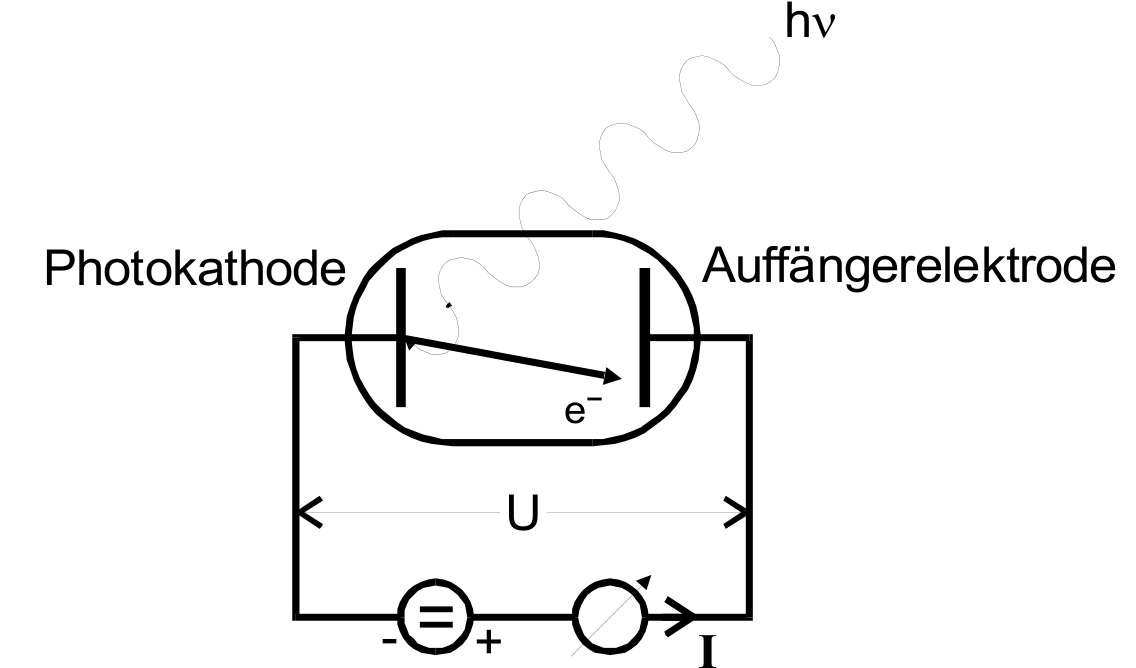
\includegraphics[height=4cm]{ressources/aufbau.png}
  \caption{Photozelle in einem Stromkreis. \cite{skript}}
  \label{abb:1}
\end{figure}

Die Photonen treffen auf die Photokathode in welcher sie Elektronen loslösen, die wiederrum von der Photoanade aufgefangen werden wodurch ein messbarer Strom erzeugt wird.
Empirisch ergeben sich somit drei Zusammenhänge.\\
Zunächst, dass Stromstärke, somit die Anzahl der aufgefangenen Elektronen proportional zur Intensität der verwendeten Strahlung ist.
Zweitens ist die kinetische Energie der Elektronen proportional zur Lichtfrequenz und steht in keiner Beziehung zur Lichtintensität.
Zuletzt, dass erst Licht ab einer gewissen Frequenz nötig ist, um den Photoeffekt zu beobachten.\\
Dabei ist zu erwähnen, dass sich diese Phänomene nicht mit dem üblichen Wellenmodell des Lichtes erklären lassen.
Wird davon ausgegangen, dass die Elektronen von den Lichtwellen zu Schwingungen angeregt werden, müsste der Photoeffekt nach einer gewissen Zeit auch bei Licht geringer Frequenz beobachtet werden.
Geschweige dessen, dass Resonanzeffekte zu bevorzugten Situationen führen würde, unter denen der Photoeffekt auftritt.\\
Einstein folgerte, dass jene Lichtteilchen gleich den Planckschen Energiequanten sind.
Im Bezug auf den Photoeffekt ergibt sich im Voraus die Erkenntnis, dass monochromatisches Licht der Frequenz $\nu$ aus Photonen der Energie
\begin{equation}
  E_{\text{ph}} = h \nu
\end{equation}
besteht, wobei $h$ das Plancksche Wirkungsquantum ist.
Trifft nun dieses Lichtteilchen auf ein Elektron im Material, so gibt es seine Energie ab.
Die gewonnene Energie teilt sich in einen Teil $A$, den das Elektron braucht, um sich vom Material zu lösen, und einen kinetischen Teil auf,
\begin{equation}
  \label{eqn:bla}
  h \nu = A + E_{\text{kin}}.
\end{equation}
Bei dem Wechselwirkungsprozess verschwindet das Photon, da es seine ganze Energie an das Elektron abgibt.
Die Gleichung sagt außerdem aus, dass der Photoeffekt nur beobachtbar ist, wenn die Energie des Photons mindestens die Austrittsarbeit tilgen kann.

% 2x2 Plot
% \begin{figure*}
%     \centering
%     \begin{subfigure}[b]{0.475\textwidth}
%         \centering
%         \includegraphics[width=\textwidth]{Abbildungen/Schaltung1.pdf}
%         \caption[]%
%         {{\small Schaltung 1.}}
%         \label{fig:Schaltung1}
%     \end{subfigure}
%     \hfill
%     \begin{subfigure}[b]{0.475\textwidth}
%         \centering
%         \includegraphics[width=\textwidth]{Abbildungen/Schaltung2.pdf}
%         \caption[]%
%         {{\small Schaltung 2.}}
%         \label{fig:Schaltung2}
%     \end{subfigure}
%     \vskip\baselineskip
%     \begin{subfigure}[b]{0.475\textwidth}
%         \centering
%         \includegraphics[width=\textwidth]{Abbildungen/Schaltung4.pdf}    % Zahlen vertauscht ... -.-
%         \caption[]%
%         {{\small Schaltung 3.}}
%         \label{fig:Schaltung3}
%     \end{subfigure}
%     \quad
%     \begin{subfigure}[b]{0.475\textwidth}
%         \centering
%         \includegraphics[width=\textwidth]{Abbildungen/Schaltung3.pdf}
%         \caption[]%
%         {{\small Schaltung 4.}}
%         \label{fig:Schaltung4}
%     \end{subfigure}
%     \caption[]
%     {Ersatzschaltbilder der verschiedenen Teilaufgaben.}
%     \label{fig:Schaltungen}
% \end{figure*}
